After a model is trained, the first step is model selection and assessment.
Selection is estimating model performance among a set of trained models using a
single validation set.  After one model is chosen, assessment takes place by
determining the prediction capability on new data via a previously unseen
testing set. Both selection and assessment can be done in a single step using
\textit{k}-fold cross-validation, which is described below.

\subsubsection{Sources of Error} 

In statistical learning, there are two sources of error that need to be
simultaneously minimized: bias and variance. Bias is caused by simplifications
in the model, so the error is caused by missed relationships in the data; an
underfit model is due to high bias.  Variance is caused by including random
noise in the model, so the error is caused by oversensitivity to that noise; an
overfit model is due to high variance. 

%%%%%%%%%%%%%%%%%%%%%%%%%%%%%%%%%%%%%%%%%%%%%%%%%%%%%%%%%%%%
%%%%%%%%%%%%%%%%%%%%%%%%%%%%%%%%%%%%%%%%%%%%%%%%%%%%%%%%%%%%
Include math or just reference it?
Talk about irreducible error too?
%%%%%%%%%%%%%%%%%%%%%%%%%%%%%%%%%%%%%%%%%%%%%%%%%%%%%%%%%%%%
%%%%%%%%%%%%%%%%%%%%%%%%%%%%%%%%%%%%%%%%%%%%%%%%%%%%%%%%%%%%

\begin{figure}[!htb]
  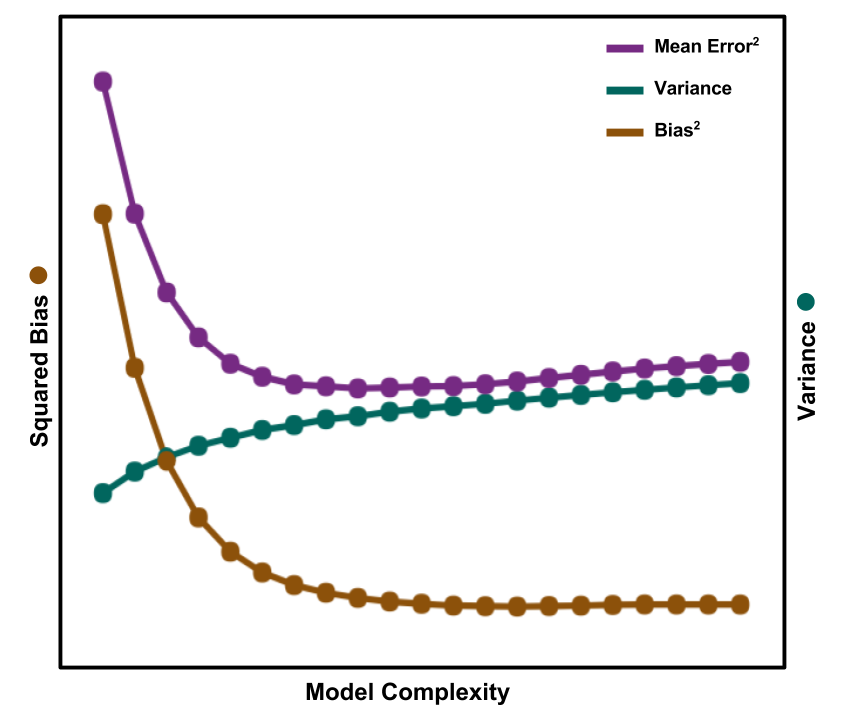
\includegraphics[width=\linewidth]{./chapters/litrev/BVtradeoff.png}
  \caption{Total prediction error comprised of bias and variance}
  \label{fig:bvtradeoff}
\end{figure}

As shown in Figure \ref{fig:bvtradeoff}, there is a minimum in the total error,
showing that there is a tradeoff between the bias and variance. Some bias is
desired in order to generalize to future unknown data. But some variance is
also positive for the model because it captures the relationships in the data
that the bias counteracts. 

\subsubsection{Types of Error}

While the sources of the model prediction error are well known, the creation of
a statistically learned model is a hidden process. Although the model emerges
from a black box, there are ways to evaluate the generalization (i.e.,
prediction) capability of it.  This is done by removing a small portion of the
data for use as a testing set.  The rest of the data set is known as the
training set and is used to train a model. After training, the test set is used
to test the model.  

The generalization error is typically referred to as the \textit{testing
error}, as it is measuring the ability of the model to predict future cases
that were not introduced in the training phase (i.e., the testing set entries).
Next, the \textit{training error} is provided by comparing the model
predictions to the training set, as the model would likely be smoother than the
potential noise the training set would include. This is useful to determine the
fitness of the model, the application of which is discussed below in Section
\ref{sec:optvalid}.

Although one could just train and test their model, there is a way to test the
model while still in the training phase. A testing set that would be used
during training to give feedback, a \textit{cross-validation} set, can provide
a faster convergence to a satisfactory model. As shown in Figure
\ref{fig:cverror}, this can be done by splitting the data set into three
groups: a large training set, a small cross-validation set, and a small testing
set. 

\begin{figure}[!htb]
  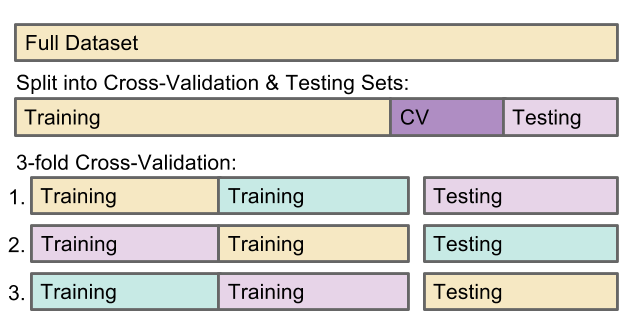
\includegraphics[width=\linewidth]{./chapters/litrev/cverror.png}
  \caption{Illustration of how a dataset can be split up for model evaluation}
  \label{fig:cverror}
\end{figure}

However, in practice, multiple rounds of cross-validation steps are used,
referred to as \textit{k-fold cross-validation}. This allows a user to use all
data entries as a testing entry once.  As illustrated in Figure
\ref{fig:cverror}, this splits the dataset into \textit{k} subsets. One set is
designated as the testing set, and a model is trained with the rest. Following
the first training phase, another begins, this time with a different subset as
the testing set.  This process is performed \textit{k} times to give \textit{k}
models, and the models are then averaged, providing an additional level of
model validation than can be achieved with a single testing set.

